 
\section{The Big Picture}

\begin{figure}
  \centering
  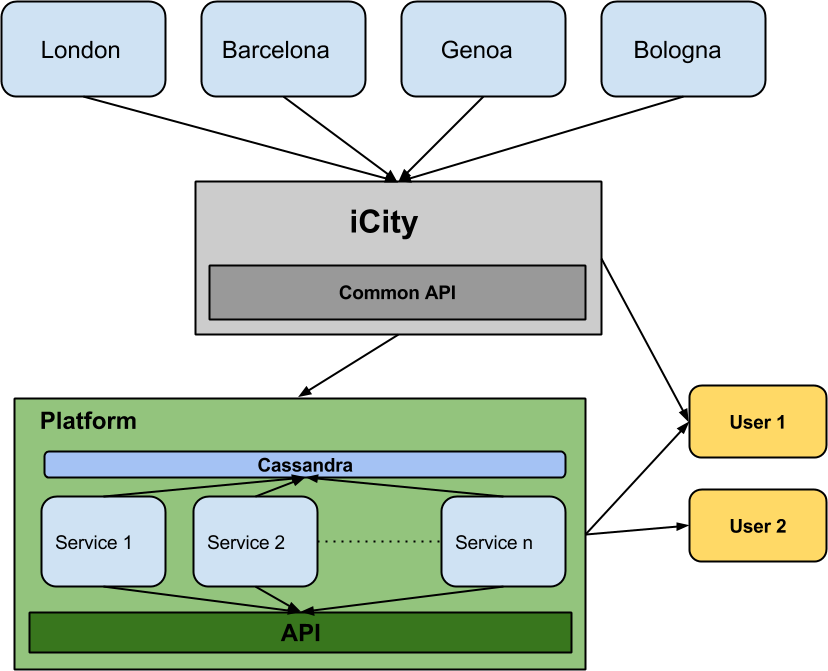
\includegraphics[scale=0.5]{overview/images/big.png}
  \caption{The architecture of the platform}\label{fig:architecture}
\end{figure}

In this section I am going to explain the architecture of the platform. It does
not enter into many details, but it is helpful in order to get a quick overview
on the design of the platform.

\begin{enumerate}
  \item The cities of London, Barcelona, Genoa and Bologna are {\bf producers}.
This list of cities will expand over time. Users are {\bf consumers}. They can
consume from either the iCity \ac{API}, from the \ac{API} from my platform, or
from both.
  \item The {\bf iCity} platform offers a common \ac{API} that integrates all
the cities. It gets the data from the different cities and allows the access of
this data to any user registered in the iCity platform.
  \item My {\bf platform} acts as a user of the iCity \ac{API} and users can
access the processed data.
  \item This platform is formed by {\bf several} services. These services
consume the data from the iCity platform in order to produce the requested
information.
  \item All the services from this platform are available through an {\bf
\ac{API}}.
  \item All the services are part of a {\bf Storm} topology.
  \item All the services share the {\bf state} of the platform, and it is stored
in a Cassandra instance.
\end{enumerate}

